\section{Logical View}
\label{sec:LogView}

In this section, I will describe the system from a high-level perspective, and get more detailed through each subsection until the entire system is described.

\subsection{High-Level Design (Scripts)}
\label{subsec:HLDesign}

The high-level view consists of a series of 6 scripts that communicate via events.
Some utilize publicly declared variables to handle logic which will be described later in subsection \ref{subsec:MLDesign}.

\begin{figure}[h]
    \centering
    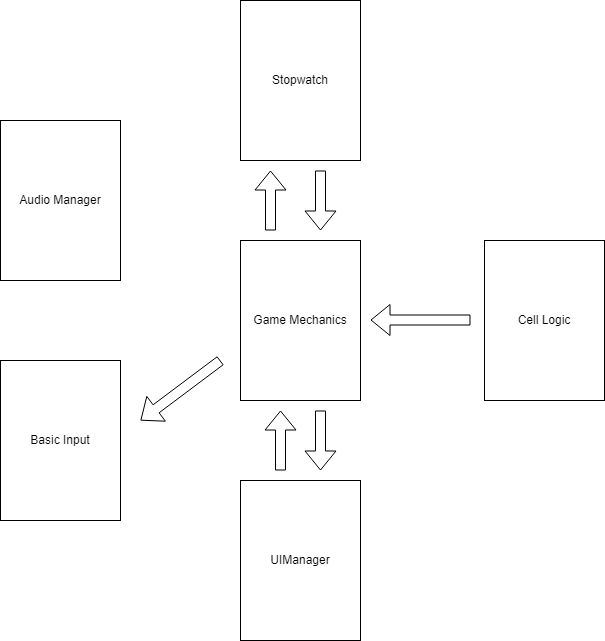
\includegraphics[width=10cm]{Images/HighLevelLogView.png}
       \caption{State Diagram describing the connectivity of the scripts.}
           \label{Fig:HighLevelLogView}
\end{figure}

\begin{itemize}
    \item The Audio Manager Script operates alone and handles volume control of the entire game.
    \item The Basic Input Script allows for the player to adjust the camera position on the game screen.
    It relies on a variable stored within Game Mechanics Script describing the player being in a game or not.
    This is because the player should only be allowed to move the camera when they are playing a game, not on a menu.
    \item The Stopwatch Script contains the logic used to maintain a stopwatch for the player when the enter the game and are playing.
    The Stopwatch only starts when the game is started, and is returned when the game is finished.
    This information gets passed to the Game Mechanics Script.
    \item The Game Mechanics Script is the heavy lifter for the entire game. 
    This handles board generation and utilizes events from other scripts to operate, whether it be screen/menu management, game state, board creation/deletion, and more.
    \item The UI Manager Script handles logic for button presses and events for menu switching.
    \item The Cell Logic Script holds the information necessary for the cells to be used within the board created within the Game Mechanics Script.
\end{itemize}

\subsection{Mid-Level Design}
\label{subsec:MLDesign}

The mid-level shows the functionality of each of the scripts and how they connect together.

\begin{figure}[h]
    \centering
    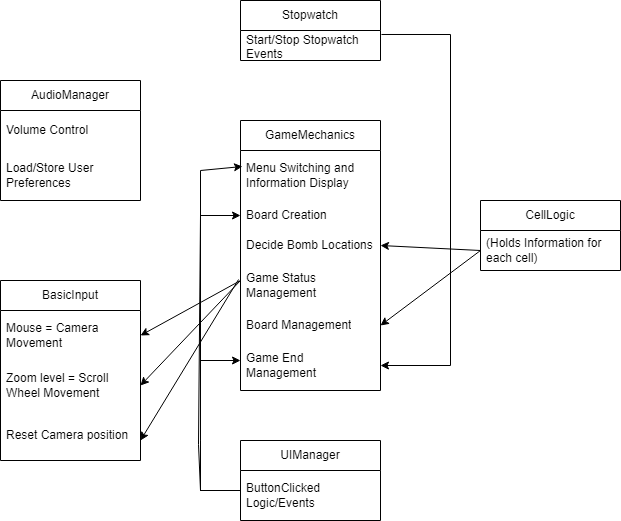
\includegraphics[width=12cm]{Images/MLDesignLogView.png}
       \caption{UML Diagram describing Mid-Level connectivity between scripts.}
           \label{Fig:MLDesignLogView}
\end{figure}

\newpage

\subsection{Detailed Class Design}
\label{subsec:DCDesign}

\begin{figure}[!htb]
    \centering
    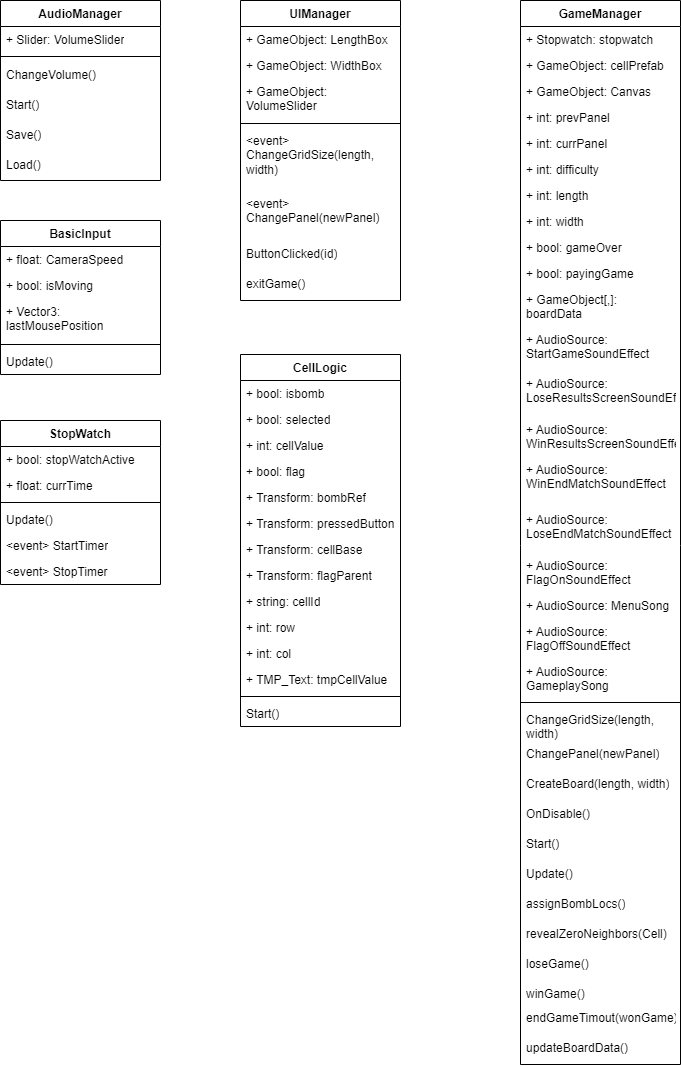
\includegraphics[width=\textwidth,height=\textheight,keepaspectratio]{Images/DCDesignLogView.png}
       \caption{UML Class Diagram for each script.}
           \label{Fig:DCDesignLogView}
\end{figure}